%
% newton.tex
%
% (c) 2020 Prof Dr Andreas Müller, Hochschule Rapperswil
%
\begin{frame}
\frametitle{Newton-Verfahren}
\begin{columns}[t]
\begin{column}{0.48\hsize}
Grenzfall des Sekanten-Verfahrens: $x_{n-1}\to x_n$
\begin{align*}
x_{n+1}
&=
x_n - f(x_n)
\underbrace{
\frac{x_n-x_{n-1}}{f(x_n)-f(x_{n-1})}}_{\displaystyle\to 1/f'(x_n)}
\\
&\uncover<2->{=
x_{n+1} - \frac{f(x_n)}{f'(x_n)}}
\end{align*}
\uncover<3->{
Vorteile:
\begin{itemize}
\item<3-> stabil
\item<4-> schnell
\end{itemize}}
\end{column}
\begin{column}{0.48\hsize}
\begin{center}
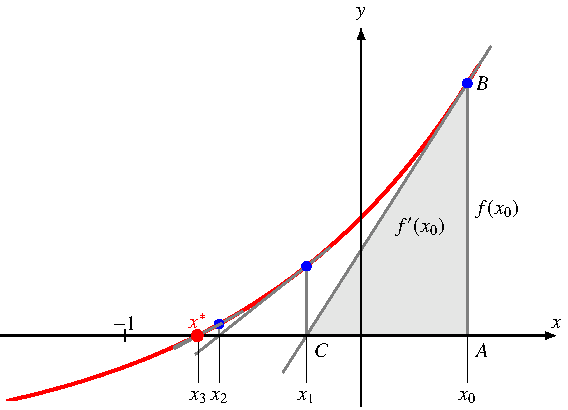
\includegraphics[width=\hsize]{../../buch/chapters/20-gleichungen/figures/newton.pdf}
\end{center}
\end{column}
\end{columns}
\end{frame}
